\documentclass[11pt,a4paper]{article}
\usepackage[margin=2cm]{geometry}
\usepackage{booktabs,tabularx,array,enumitem,xcolor,hyperref,listings,amsmath}
\usepackage[T1]{fontenc}
\usepackage{lmodern}
\usepackage{tikz}
\usetikzlibrary{automata,positioning,arrows.meta}
\hypersetup{colorlinks=true,linkcolor=blue!50!black,urlcolor=blue!50!black}
\newcolumntype{L}{>{\raggedright\arraybackslash}X}
\setlist{nosep,leftmargin=*}
\setlength{\emergencystretch}{3em}
\lstset{language=C,basicstyle=\ttfamily\footnotesize,breaklines=true,columns=fullflexible,keepspaces=true,
  frame=single,framerule=0.3pt,rulecolor=\color{black!30},xleftmargin=2pt,xrightmargin=2pt,
  commentstyle=\color{green!40!black},keywordstyle=\color{blue!60!black},showstringspaces=false}
\newcommand{\lv}[1]{\texttt{#1}}                 % a Live Expressions variable
\newcommand{\run}[1]{\textbf{How to run.} #1}
\newcommand{\see}[1]{\textbf{What you see.} #1}

\title{Microprocessor-Based Product Design 2026/27\\[2pt]\large Assignment 1: reference solution}
\author{Yohai Ackerman (TA). \textbf{TA only, never handed to students.}}
\date{Draft of \today}

\begin{document}
\maketitle

\section{The project and how to operate it}

\subsection{What is where}
Everything is in \texttt{assignments/ass1/solution/fullSolution/}:

\smallskip\noindent
\begin{tabularx}{\textwidth}{@{}l L@{}}
\toprule
File & Content \\
\midrule
\texttt{ass1\_sol.tex} & this document \\
\texttt{ass1\_sol/} & the STM32CubeIDE project \\
\texttt{ass1\_sol/ass1\_sol.ioc} & \texttt{ass1.ioc}, unchanged except the project name \\
\texttt{Core/Src/main.c} & generated code; the user code adds \texttt{\_\_io\_putchar} (printf to PuTTY, tutorial~2),
  \texttt{ioBoardInit()}, and calls the task dispatcher in the main loop \\
\texttt{Core/Src/io\_board.c}, \texttt{Core/Inc/io\_board.h} & the students' copy, unchanged \\
\texttt{Core/Inc/ass1.h} & task numbers and shared helpers \\
\texttt{Core/Src/ass1\_tasks.c} & the dispatcher: runs the task chosen in \lv{task} \\
\texttt{Core/Src/ass1\_common.c} & \texttt{printBinary}, \texttt{showByteOnLeds}, \texttt{readButtonsHeld}, the debouncer \\
\texttt{Core/Src/bits.c}, \texttt{Core/Inc/bits.h} & B.1: \texttt{bitSet}, \texttt{bitClear}, \texttt{bitToggle},
  \texttt{bitTest} \\
\texttt{Core/Src/partA.c} \ldots\ \texttt{partE.c} & one file per part \\
\bottomrule
\end{tabularx}

\subsection{Opening, building and starting a debug session}
\begin{enumerate}
  \item In STM32CubeIDE: \emph{File $\to$ Import $\to$ General $\to$ Existing Projects into Workspace}, root directory
        \texttt{fullSolution/ass1\_sol}. Build with the hammer (Debug configuration).
  \item Connect the Nucleo (power jumper on 5V\_STLK) and the IO board. Open PuTTY on the ST-LINK COM port (Device
        Manager shows the number), 115\,200 baud, 8N1.
  \item Start a debug session (\emph{Run $\to$ Debug}, or the launch file \texttt{ass1\_sol Debug.launch}) and press
        \emph{Resume} (F8). PuTTY shows the IO board report of \texttt{ioBoardInit()} (all four chips ``found'') and the
        task menu.
  \item Open \emph{Window $\to$ Show View $\to$ Live Expressions}, and add \lv{task} with \emph{Add new expression}.
        Add the other variables named in each part below.
\end{enumerate}

\subsection{Choosing a task}
All parts are in one program. The global variable \lv{task} chooses what runs: click its \emph{Value} cell in Live
Expressions while the program runs, type the number, and press Enter. The running task notices the change, returns,
the LEDs and LD2 are switched off, and the new task starts (PuTTY prints \texttt{=== task N ===}). To restart the same
task (for example after changing its settings), write \texttt{0}, then the number again.

\smallskip\noindent
\begin{tabularx}{\textwidth}{@{}c L c L@{}}
\toprule
\lv{task} & Runs & \lv{task} & Runs \\
\midrule
0  & idle (start-up value) & 31 & C.1 level-based counting \\
11 & A.1 wrap-around & 32 & C.2 edge-based counting \\
12 & A.2 hex values, signed and unsigned & 33 & C.3 debounced counting \\
13 & A.3 integer division & 34 & C.4 debounced counter with \texttt{HAL\_Delay(150)} \\
21 & B.1 bit functions on LD2 & 35 & C.4 edge counter with \texttt{HAL\_Delay(150)} \\
22 & B.2 one LED walks & 41 & D.1 200 toggles, timed \\
23 & B.3 a pair of LEDs walks & 42 & D.2 LD2 at a rate from a variable \\
24 & B.4 buttons held & 43 & D.3 with \texttt{HAL\_Delay} \\
   &  & 44 & D.3 with \texttt{HAL\_GetTick} \\
   &  & 51 & E armed state, IR sensor, brightening \\
\bottomrule
\end{tabularx}

\smallskip\noindent
Live Expressions shows a value in decimal by default; for the bit patterns of Parts A and B, right-click the
expression and choose another number format (hex or binary), where the view offers it. An \texttt{enum} variable
(\lv{eState}) is shown by name.

\subsection{Status of this solution}
The code was syntax-checked with GCC against the project's HAL headers (no errors; the only warnings are host-only:
\texttt{\%lu} with a 32-bit \texttt{uint32\_t}, which is \texttt{unsigned long} on the ARM target). It has \textbf{not
yet been built with the CubeIDE toolchain or run on the board}. The expected numbers below are calculated, or taken
from the TA measurements with the \texttt{bounceCheck400} project (2026-10-22, I2C at 400\,kHz, button~0); check them
on the board before grading against them.

\section{Shared helpers}
\begin{lstlisting}
void printBinary(uint32_t value, uint8_t nBits)   // printf has no %b
{
    for (int8_t i = (int8_t)(nBits - 1); i >= 0; i--)
    {
        putchar(bitTest(value, (uint8_t)i) ? '1' : '0');
        if ((i % 4 == 0) && (i != 0)) putchar('_');   // 1111_0000
    }
}

void showByteOnLeds(uint8_t pattern)              // LED n white while bit n is 1
{
    for (uint8_t n = 0; n < N_LEDS; n++)
    {
        uint8_t v = bitTest(pattern, n) ? LED_LEVEL : 0;
        setRGB_led(n, v, v, v);
    }
}

uint8_t readButtonsHeld(void)                     // bit n = 1 while button n is held
{
    return (uint8_t)(~readButtonsRaw()) & 0x0Fu;
}
\end{lstlisting}
One LED update by \texttt{showByteOnLeds} is 24 I2C writes, about 2\,ms at 400\,kHz; one button read is about
110\,$\mu$s.

\section{Part A: variable types, signed and unsigned, wrap-around}

\subsection*{A.1}
\run{Add \lv{a1U8}, \lv{a1I8}, \lv{a1U16}. Write \lv{task} = 11. The three variables start close to their limits
(\lv{a1StartU8} = 248, \lv{a1StartI8} = 124, \lv{a1StartU16} = 65530) and grow by one every \lv{a1StepMs} = 500\,ms.
After a wrap there is an extra pause of \lv{a1WrapPauseMs} = 3000\,ms, and PuTTY marks the line with
\texttt{<{}< wrap-around}. To start from other values, change the start variables, then write \lv{task} = 0 and 11.}

\see{For example:}
\begin{lstlisting}[language={},basicstyle=\ttfamily\scriptsize]
u8 255 0xFF 1111_1111 | i8  127 0x7F 0111_1111 | u16 65535 0xFFFF 1111_1111_1111_1111
u8   0 0x00 0000_0000 | i8 -128 0x80 1000_0000 | u16     0 0x0000 0000_0000_0000_0000   << wrap-around
\end{lstlisting}
(with the default start values the three wraps come at different steps).

\textbf{Answer.} An $n$-bit variable holds $2^n$ bit patterns. Adding 1 to the largest pattern (all ones) gives a
carry out of the top bit, which has no place to go and is lost, so the result is all zeros:
\begin{itemize}
  \item \texttt{uint8\_t}: $255 + 1 \to 0$; \texttt{uint16\_t}: $65\,535 + 1 \to 0$. Unsigned arithmetic in C is
        defined modulo $2^n$.
  \item \texttt{int8\_t}: $127 + 1 \to -128$. The pattern goes from \texttt{0111\_1111} to \texttt{1000\_0000}; in two's
        complement the top bit has the weight $-128$, so the same pattern now reads as $-128$. (In C the
        \texttt{int8\_t} is first promoted to \texttt{int}, $127 + 1 = 128$ is computed, and converting 128 back into an
        \texttt{int8\_t} wraps it; GCC defines this conversion as modulo $2^8$.)
\end{itemize}
The binary output shows it directly: the same 8 bits, read as unsigned or signed.

\subsection*{A.2}
\run{Write \lv{task} = 12. The table is printed once. The six variables (\lv{a2U8\_7F}, \lv{a2I8\_7F}, \lv{a2U8\_F0},
\lv{a2I8\_F0}, \lv{a2U16}, \lv{a2I16}) can also be watched in Live Expressions.}

\see{}
\begin{lstlisting}[language={},basicstyle=\ttfamily\scriptsize]
0x7F   as uint8_t      dec    127   hex 0x7F     bin 0111_1111
0x7F   as int8_t       dec    127   hex 0x7F     bin 0111_1111   (%X of the value itself: 0x7F)
0xF0   as uint8_t      dec    240   hex 0xF0     bin 1111_0000
0xF0   as int8_t       dec    -16   hex 0xF0     bin 1111_0000   (%X of the value itself: 0xFFFFFFF0)
0xFFF6 as uint16_t     dec  65526   hex 0xFFF6   bin 1111_1111_1111_0110
0xFFF6 as int16_t      dec    -10   hex 0xFFF6   bin 1111_1111_1111_0110   (%X of the value itself: 0xFFFFFFF6)
\end{lstlisting}

\textbf{Answer.} A hex digit is 4 bits, and the value is $\sum d_k\,16^k$: \texttt{0xF0} $= 15 \cdot 16 + 0 = 240$,
\texttt{0xFFF6} $= 65\,526$. For an unsigned type that is the value. For a signed type of $n$ bits, if the top bit is
1 (the first hex digit is 8 or more), the value is negative: subtract $2^n$. So \texttt{0xF0} as \texttt{int8\_t} is
$240 - 256 = -16$, \texttt{0xFFF6} as \texttt{int16\_t} is $65\,526 - 65\,536 = -10$, and \texttt{0x7F} (top bit 0)
is 127 in both types.

\emph{A negative value printed in hex:} \texttt{printf("\%X", x)} with \texttt{x = -16} prints \texttt{FFFFFFF0}, not
\texttt{F0}. A variable narrower than \texttt{int} is promoted to a 32-bit \texttt{int} when it is passed to
\texttt{printf}; a negative value is sign-extended (the top bit is copied into the 24 new bits), and \texttt{\%X}
prints all 32 bits. Casting to the unsigned type of the same width, \texttt{(uint8\_t)x}, prints \texttt{F0}.

\emph{Note:} \texttt{int8\_t x = 0xF0;} makes GCC warn (``overflow in conversion from int to int8\_t changes value
from 240 to $-16$''): the constant 240 does not fit. The solution writes \texttt{(int8\_t)0xF0} to say it is meant.

\subsection*{A.3}
\run{Write \lv{task} = 13. Watch \lv{a3AvgWrong} and \lv{a3AvgRight}. To try other grades, change \lv{a3Grade1},
\lv{a3Grade2}, then write \lv{task} = 0 and 13.}
\begin{lstlisting}
a3AvgWrong = (a3Grade1 + a3Grade2) / 2;      // 155 / 2 = 77   (integer division)
a3AvgRight = (a3Grade1 + a3Grade2) / 2.0f;   // 155 / 2.0 = 77.5
\end{lstlisting}
\textbf{Answer.} When both operands of \texttt{/} are integers, C does an integer division, and the fraction is
dropped: 77 instead of 77.5. If either operand is a floating-point value (\texttt{2.0f}, or a cast
\texttt{(float)(a + b) / 2}), the other is converted and the division is done in floating point. Storing the
integer result in a \texttt{float} afterwards (\texttt{float avg = (a + b) / 2;}) does not help: the fraction is
already lost. The sum itself is safe: two \texttt{uint8\_t} are promoted to \texttt{int} before the addition, so
$97 + 58 = 155$ is computed in 32 bits (storing it in a \texttt{uint8\_t} would wrap only above 255).

\emph{Printing a float:} with the default newlib-nano library, \texttt{printf("\%f")} prints nothing until
\emph{Project Properties $\to$ C/C++ Build $\to$ Settings $\to$ MCU Settings $\to$ ``Use float with printf from
newlib-nano''} is ticked. The solution avoids it and prints the tenths by hand; Live Expressions shows
\lv{a3AvgRight} = 77.5 either way.

\section{Part B: bit operations and shifting}

\subsection*{B.1}
\begin{lstlisting}
uint32_t bitSet(uint32_t value, uint8_t bit)    { return value |  (1UL << bit); }
uint32_t bitClear(uint32_t value, uint8_t bit)  { return value & ~(1UL << bit); }
uint32_t bitToggle(uint32_t value, uint8_t bit) { return value ^  (1UL << bit); }
uint8_t  bitTest(uint32_t value, uint8_t bit)   { return (uint8_t)((value >> bit) & 1UL); }
\end{lstlisting}
\run{Write \lv{task} = 21. The sequence runs once: LD2 off; after 1\,s on (set); after 1\,s off (clear); after 1\,s on
(toggle). Then \texttt{bitTest(GPIOA->ODR, 5)} = 1 lights LED~0 of the IO board (white), and \lv{b1Result} = 1. To
see it again, write \lv{task} = 0 and 21.}

\textbf{Answer.} OR with a mask sets the bit, AND with the inverted mask clears it, XOR flips it, and shifting the bit
down to bit~0 and masking with 1 tests it. The mask is \texttt{1UL << bit}: \texttt{1UL} is 32 bits wide and unsigned,
so even bit~31 of a register is safe. \texttt{GPIOA->ODR = bitSet(GPIOA->ODR, 5)} reads the output register, changes
bit~5 only, and writes it back, so the other pins of port~A keep their levels.

\subsection*{B.2 and B.3}
\begin{lstlisting}
b2Pattern = (uint8_t)((b2Pattern << 1) | (b2Pattern >> 7));   // rotate left by one
\end{lstlisting}
\run{Write \lv{task} = 22 (B.2, starts from \texttt{0x01}) or 23 (B.3, starts from \texttt{0x03}). Watch
\lv{b2Pattern}. One step per second, forever, until \lv{task} changes.}

\see{B.2: \texttt{0000\_0001}, \texttt{0000\_0010}, \ldots, \texttt{1000\_0000}, \texttt{0000\_0001}, \ldots\ B.3:
\texttt{0000\_0011}, \texttt{0000\_0110}, \ldots, \texttt{1100\_0000}, \texttt{1000\_0001} (LEDs 7 and 0),
\texttt{0000\_0011}, \ldots}

\textbf{Answer (past bit 7).} \texttt{p << 1} moves every bit one place up; bit~7 moves to bit~8, which does not
exist in a \texttt{uint8\_t} and is dropped by the cast. \texttt{p >> 7} moves that same bit~7 down to bit~0 (all the
other bits fall off the right). OR joins the two results, so the bit that leaves at the top comes back at the bottom:
a rotation. No \texttt{if}, no counter and no table is needed, and the same line serves one lit LED or two. The LEDs
are lit by \texttt{showByteOnLeds}, which tests each bit.

\subsection*{B.4}
\run{Write \lv{task} = 24. Watch \lv{b4Raw}, \lv{b4Held} and \lv{b4Count}. Hold any combination of the four buttons.}

\see{With button~0 held: \texttt{raw 0b1111\_1110 held 0b0000\_0001 -> 1 button(s) held}. With buttons 0 and 2:
\texttt{held 0b0000\_0101 -> 2}. A line is printed only when the count changes.}

\textbf{Answer.} The buttons are active-low, so \texttt{\textasciitilde raw} makes a held button a 1. Bits 4 to 7 of
the PCA9538A carry no button; after the inversion they may be 0 or 1, so \texttt{\& 0x0F} clears them. The count is
the sum of \texttt{bitTest(held, n)} for $n = 0$ to 3.

\section{Part C: input triggering}
\run{In every version, watch \lv{cCount}. The count is shown on the 8 LEDs (its lowest 8 bits) and printed only when it
changes. To start a new round of 20 presses, write \lv{cReset} = 1 (it returns to 0 by itself, and the count to 0).
Write \lv{task} = 31, 32, 33, 34 or 35 for C.1, C.2, C.3, C.4 (debounced) and C.4 (edge). \lv{cDebounceMs} = 20 and
\lv{cDelayMs} = 150 can be changed while it runs.}

\subsection*{C.1 Level-based}
\begin{lstlisting}
uint8_t now = bitTest(readButtonsHeld(), 0);
if (now) cCount++;                       // every pass while held
if (before && !now) showCount();         // shown once, when the button is released
before = now;
\end{lstlisting}
Also watch \lv{cLoopsPerSec}, printed once a second.

\textbf{Expected.} About 9\,000 loop passes per second: one pass is one I2C read of the button chip, about
110\,$\mu$s. A press of about 150\,ms adds about $0.15 \times 9000 \approx 1\,350$, so 20 presses give a count of
tens of thousands, different every round (the LEDs show only its lowest 8 bits). \textbf{Answer:} the level-based
counter counts loop passes while the button is held, not presses; the count is
(passes per second) $\times$ (total time held).

\subsection*{C.2 Edge-based}
\begin{lstlisting}
uint8_t now     = readButtonsHeld();
uint8_t pressed = now & (uint8_t)~before;   // 1 where a button went from released to pressed
before = now;
if (bitTest(pressed, 0)) { cCount++; showCount(); }
\end{lstlisting}
\textbf{Expected} (TA measurement): natural presses 20 to 23 per 20; very light, slow presses about 26 per 20.
\textbf{Answer:} a mechanical contact bounces: while it closes or opens, it makes and breaks contact several times
within about a millisecond. A read that falls in such a gap sees ``released'', the next one ``pressed'', and the edge
counter counts an extra press. The bounce pulses are shorter than one read (110\,$\mu$s), so only some are caught,
and the count is sometimes 20, sometimes more. A light, slow press keeps the contact near its switching point for
longer, so it bounces more.

\subsection*{C.3 Debounced}
\begin{lstlisting}
uint8_t debounceUpdate(Debouncer *d, uint8_t sample, uint32_t tick, uint32_t stableMs)
{
    if (sample != d->raw) { d->raw = sample; d->changeTick = tick; }      // moved: restart
    else if ((sample != d->stable) && (tick - d->changeTick >= stableMs))
    {
        d->stable = sample;                 // stable for 20 ms: accept
        return sample;                      // 1 only for an accepted press
    }
    return 0;
}
\end{lstlisting}
\textbf{Expected:} 20 of 20 in every round, light presses too. A bounce gap restarts the 20\,ms timer, so the new state
is accepted only once the contact has settled.

\subsection*{C.4 Missing presses}
\textbf{Expected} (TA measurement, quick taps of 110 to 130\,ms, \texttt{HAL\_Delay(150)}): debounced (34) 0 of 20,
edge (35) about 11 of 20.

\textbf{Answer.} With the delay, the button is read once per loop pass, about 151\,ms (\texttt{HAL\_Delay(150)} waits
at least 150\,ms and up to 151, plus 0.1\,ms for the read). A tap shorter than that is seen by at most one read, or by
none if it falls between two reads. The edge version needs one read inside the tap, so it catches a tap with a
probability of about (tap duration) / (loop period), and loses the rest. The debounced version needs the pressed state
to be seen again at least 20\,ms later; the next read comes 151\,ms later, when a quick tap is already over, so the
change is never confirmed and it loses all of them. In general, a reliable reading needs a loop period much shorter
than the shortest input event: here the ``other task'' of 150\,ms makes that impossible, and the cure is to keep the
loop short (non-blocking code, Part~D) or to let the input interrupt the program (EXTI, Assignment~2).

\smallskip\noindent
\begin{tabularx}{\textwidth}{@{}l c c c L@{}}
\toprule
Version & Round 1 & Round 2 & Round 3 & Expected \\
\midrule
C.1 level & & & & tens of thousands, different each round \\
C.2 edge, natural & & & & 20 to 23 \\
C.2 edge, light & & & & about 26 \\
C.3 debounced & & & & 20 \\
C.4 debounced + delay & & & & 0 \\
C.4 edge + delay & & & & about 11 \\
\bottomrule
\end{tabularx}

\section{Part D: LED blinking and timing}
\run{Part D is one program with the rest. D.1: write \lv{task} = 41; watch \lv{d1Toggles} and \lv{d1TotalMs}; it
stops by itself after 200 toggles, and prints the total. D.2: write \lv{task} = 42, then change
\lv{d2HalfPeriodMs} (default 500) while LD2 blinks. D.3: write \lv{task} = 43 (\texttt{HAL\_Delay}) or 44
(\texttt{HAL\_GetTick}); watch \lv{d3Led0Ms} and \lv{d3Led1Ms}, which hold the last measured time for 10 blinks of
each LED, also printed. The rates are \lv{d3FreqMilliHz0} = 1000 and \lv{d3FreqMilliHz1} = 1300 (in mHz).}

\subsection*{D.1}
\begin{lstlisting}
for (d1Toggles = 0; d1Toggles < 200; )
{
    HAL_GPIO_TogglePin(LD2_GPIO_Port, LD2_Pin);
    d1Toggles++;
    printf("D.1 toggle %3lu of 200   t = %6lu ms   LD2 = %u  status OK\r\n", ...);  // 60 characters
    HAL_Delay(500);
}
d1TotalMs = HAL_GetTick() - start;
\end{lstlisting}
\textbf{Expected:} $200 \times 500\,\text{ms} = 100\,000$\,ms by calculation; measured about 101\,200\,ms.

\textbf{Answer.} Two things add to the 500\,ms:
\begin{itemize}
  \item The UART. \texttt{printf} sends the line through \texttt{HAL\_UART\_Transmit}, which waits until each character
        has left. One character is 10 bits (start, 8 data, stop): $10 / 115\,200 = 86.8\,\mu$s. A 60-character line
        takes $60 \times 86.8\,\mu\text{s} = 5.2$\,ms, during which the program does nothing else.
  \item \texttt{HAL\_Delay} adds one tick to guarantee the minimum wait (the line \texttt{wait += uwTickFreq}
        in \texttt{stm32g4xx\_hal.c}), so \texttt{HAL\_Delay(500)} waits until 501 ticks have passed.
\end{itemize}
Together, each pass ends 501 ticks after the tick in which the print ended, which is 5 ticks after the pass began:
$5 + 501 = 506$\,ms per pass, and $200 \times 506 = 101\,200$\,ms, 1.2\% more than calculated.

\subsection*{D.2}
\begin{lstlisting}
while (task == TASK_D2)
{
    HAL_GPIO_TogglePin(LD2_GPIO_Port, LD2_Pin);
    HAL_Delay(d2HalfPeriodMs);              // read again every half period
}
\end{lstlisting}
The blink frequency is $f = 1000 / (2\,(d + 1))$\,Hz for \lv{d2HalfPeriodMs} $= d$ (the $+1$ is again
\texttt{HAL\_Delay}): 500 gives 0.998\,Hz, 100 gives 4.95\,Hz, 50 gives 9.8\,Hz. A new value takes effect at the next
toggle.

\subsection*{D.3}
Theory: one blink is one on and one off, so 10 blinks take 10 periods: LED~0 (1\,Hz) $10 \times 1\,\text{s} =
10\,000$\,ms, LED~1 (1.3\,Hz) $10 / 1.3 = 7\,692$\,ms. Each half period: 500\,ms and 384.6\,ms. The time is measured
from the toggle that starts blink~1 to the toggle that starts blink~11.

\paragraph{With \texttt{HAL\_Delay} (task 43).}
\begin{lstlisting}
blinkerToggle(&led0, &d3Led0Ms);   HAL_Delay(500);
blinkerToggle(&led1, &d3Led1Ms);   HAL_Delay(385);
\end{lstlisting}
\textbf{Expected:} about 17\,740\,ms for \emph{both} LEDs. Each pass toggles each LED once and waits for both delays,
$501 + 386 = 887$\,ms (the toggles themselves, 3 I2C writes each, about 0.25\,ms, fall inside the same ticks); 10
blinks are 20 passes. \textbf{Answer:} with blocking delays the two LEDs cannot have their own rates: the program
waits for one LED while the other one is due, so both LEDs blink at the rate set by the sum of the delays, 0.56\,Hz
instead of 1 and 1.3\,Hz.

\paragraph{With \texttt{HAL\_GetTick} (task 44).}
\begin{lstlisting}
uint32_t nowUs = HAL_GetTick() * 1000u;
if ((int32_t)(nowUs - next0) >= 0) { blinkerToggle(&led0, &d3Led0Ms); next0 += 500000; }
if ((int32_t)(nowUs - next1) >= 0) { blinkerToggle(&led1, &d3Led1Ms); next1 += 384615; }
\end{lstlisting}
\textbf{Expected:} LED~0 10\,000\,ms, LED~1 7\,692 or 7\,693\,ms (within 1\,ms of the theory).
\textbf{Answer:} each LED has its own deadline, and the loop never waits, so each LED toggles within one tick of its
deadline, whatever the other does. Three details decide the accuracy, and are the differences students are expected
to find:
\begin{itemize}
  \item Advance the deadline by the period (\texttt{next += half}), not to ``now'' (\texttt{last = now}). With
        \texttt{last = now}, every toggle starts its wait from the moment it was noticed, up to 1\,ms late plus the
        I2C write, and the errors add up over 20 toggles.
  \item The half period of 1.3\,Hz is 384.615\,ms, not a whole number of ticks. A deadline in whole ms (385) gives
        $20 \times 385 = 7\,700$\,ms, 8\,ms (0.1\%) too long. Keeping the deadlines in microseconds lets the toggles
        fall on 384 or 385\,ms, so that the average is right.
  \item The tick is 1\,ms, so a single toggle can be up to 1\,ms off; that does not add up when the deadline is
        advanced by the period.
\end{itemize}
The subtraction \texttt{nowUs - next} is converted to a signed number, so the comparison stays right when the counter
wraps (Part~A again).

\smallskip\noindent
\begin{tabularx}{\textwidth}{@{}l c c L@{}}
\toprule
 & LED 0, 1\,Hz & LED 1, 1.3\,Hz & Why \\
\midrule
Theory & 10\,000\,ms & 7\,692\,ms & 10 periods \\
\texttt{HAL\_Delay} & about 17\,740\,ms & about 17\,740\,ms & both delays in every pass \\
\texttt{HAL\_GetTick}, ms deadlines & 10\,000\,ms & 7\,700\,ms & 385 instead of 384.6\,ms \\
\texttt{HAL\_GetTick}, $\mu$s deadlines (this solution) & 10\,000\,ms & 7\,692\,ms & within one tick \\
\bottomrule
\end{tabularx}

\section{Part E: integration and logic}
\run{Write \lv{task} = 51. Watch \lv{eArmed}, \lv{eObstacle}, \lv{eCondition}, \lv{eState} and \lv{eLevel}. Button~0
arms and disarms (LD2 is on while armed). Hold a hand in front of the IR sensor for an obstacle. \lv{eStepMs} = 40 and
\lv{eStepSize} = 5 give 51 steps of 40\,ms, about 2\,s from off to full; \lv{eUseGamma} = 1 makes the steps look even
to the eye (\texttt{gamma2} of \texttt{io\_board.h}), 0 gives linear values.}

\paragraph{Truth table of the trigger condition.}
\begin{center}
\begin{tabular}{c c c}
\toprule
armed & obstacle & condition \\
\midrule
0 & 0 & 0 \\
0 & 1 & 0 \\
1 & 0 & 0 \\
1 & 1 & 1 \\
\bottomrule
\end{tabular}
\end{center}

\paragraph{State diagram.}
\begin{center}
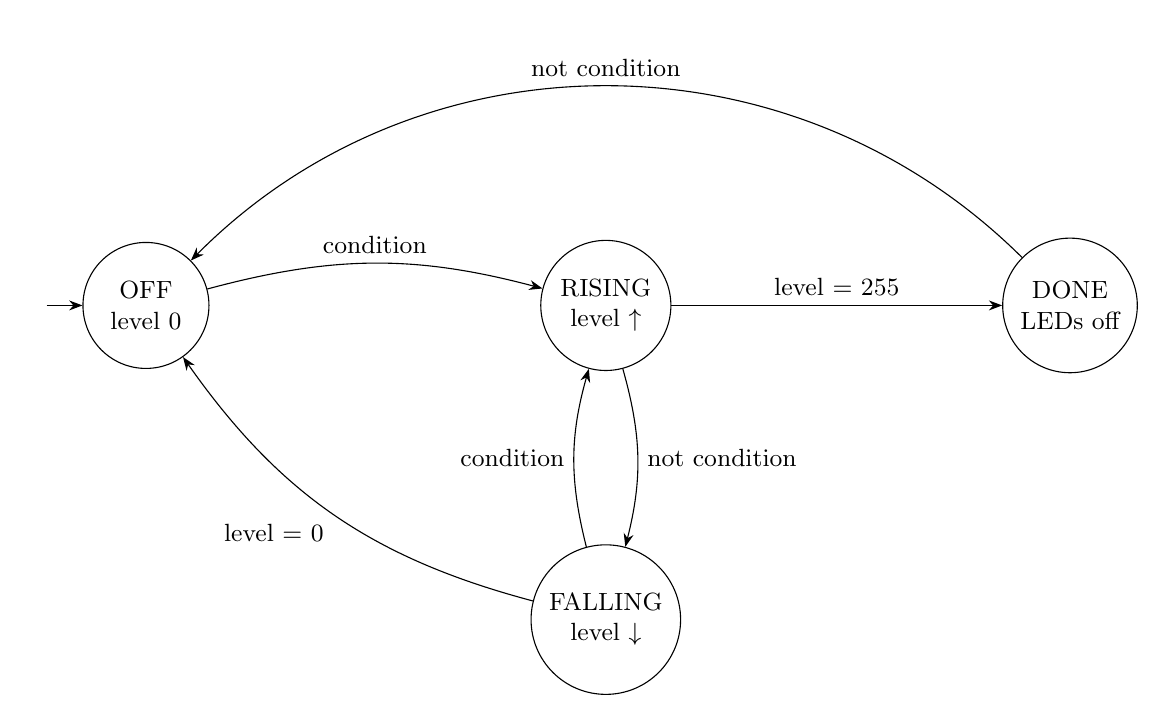
\begin{tikzpicture}[>=Stealth,node distance=2.2cm and 4.2cm,every state/.style={minimum size=1.6cm,align=center,font=\small},
  every edge/.style={draw,->},font=\small]
  \node[state,initial,initial text={}] (off) {OFF\\level 0};
  \node[state,right=of off] (rise) {RISING\\level $\uparrow$};
  \node[state,below=of rise] (fall) {FALLING\\level $\downarrow$};
  \node[state,right=of rise] (done) {DONE\\LEDs off};
  \path (off)  edge[bend left=15] node[above] {condition} (rise)
        (rise) edge node[above] {level = 255} (done)
        (rise) edge[bend left=15] node[right] {not condition} (fall)
        (fall) edge[bend left=15] node[left] {condition} (rise)
        (fall) edge[bend left=20] node[below left] {level = 0} (off)
        (done) edge[bend right=45] node[above] {not condition} (off);
\end{tikzpicture}
\end{center}
In RISING the level grows by \lv{eStepSize} every \lv{eStepMs}; when 255 has been shown for one step, the LEDs switch
off (DONE), and stay off until the condition is false (back to OFF) and then true again. In FALLING the level drops by
one step every \lv{eStepMs}, from wherever it was, down to 0. The assignment does not say what happens if the condition
returns during the dimming; this solution brightens again from the current level.

\paragraph{The main loop.} The button (debounced, as in C.3) and the IR sensor are read on every pass; the state
changes as soon as the condition changes; the brightness steps are paced by \texttt{HAL\_GetTick}. Nothing waits, so
an obstacle or a press is never missed (compare C.4).

\paragraph{Test sequence} (also the content of the video \texttt{V\_E}):
\begin{enumerate}
  \item Disarmed, obstacle: nothing happens (condition 0).
  \item Arm (LD2 on), no obstacle: nothing happens.
  \item Armed, hold the obstacle: the LEDs brighten for about 2\,s, then switch off (DONE). Keep the hand there: they stay
        off.
  \item Remove the hand (OFF) and bring it back: a new brightening.
  \item Remove the hand halfway through: the LEDs dim from their current level to off.
  \item Disarm with the button halfway through a brightening: the LEDs dim (the condition is false).
\end{enumerate}

\section{Grading notes}
\begin{itemize}
  \item A.1: the wrap must be visible both in Live Expressions and in PuTTY, in three formats; binary needs a
        function of their own. A.2: the explanation of \texttt{FFFFFFF0} (promotion and sign extension) is the key point.
  \item B.2 and B.3: patterns chosen with \texttt{if}/\texttt{switch}, a counter mapped to LEDs, or a table, are not
        accepted (the rule in the assignment). The rotation line, or an equivalent \texttt{if (p \& 0x80)} that then uses
        only bit operations, is.
  \item C: the explanation must use the press duration and the loop time.
  \item D.1: both the UART time (5.2\,ms per line) and the extra tick of \texttt{HAL\_Delay} explain the difference; the
        UART is the larger one.
  \item D.3: the blocking version must show that both LEDs end up at the same rate; the non-blocking version must be
        within a few ms of the theory, and the report must explain any remaining difference.
  \item E: the inputs must be read on every pass (no \texttt{HAL\_Delay} in the stepping); the truth table and a state
        diagram with the condition on every transition are required.
\end{itemize}

\end{document}
